\documentclass[12pt,a4paper]{article}
\usepackage[margin=2.4cm]{geometry}
\usepackage{fontspec}
\setmainfont{Times New Roman}
\usepackage{longtable,booktabs,array,enumitem,tikz,hyperref,graphicx,xcolor,fancyhdr}
\usetikzlibrary{positioning,shapes.geometric}
\definecolor{CoverBlue}{HTML}{263CBF}
\hypersetup{hidelinks,pdftitle={BrewLite - Bao cao Assignment 2}}
\setlength{\parskip}{0.4em}
\setlength{\parindent}{0pt}
\setlist[itemize]{nosep,leftmargin=2em}
\renewcommand{\contentsname}{Mục lục}
\pagestyle{fancy}
\fancyhf{}
\fancyfoot[L]{\small BrewLite -- Assignment 2}
\fancyfoot[R]{\small\thepage}
\renewcommand{\headrulewidth}{0pt}
\begin{document}
% Bìa theo bố cục báo cáo Assignment 1 của nhóm, cập nhật cho Assignment 2.
\hypersetup{pageanchor=false}
\begin{titlepage}
  \thispagestyle{empty}
  \begin{center}
    {\normalsize TRƯỜNG ĐẠI HỌC SÀI GÒN}\\[3pt]
    {\normalsize KHOA CÔNG NGHỆ THÔNG TIN}\\[16mm]
    
\includegraphics[width=32mm]{logoITSGU.png}
  \end{center}

  \vspace{11mm}
  \begin{center}
    \color{CoverBlue}
    {\Large\bfseries CÔNG NGHỆ PHẦN MỀM}\\[3mm]
    \rule{\textwidth}{0.5pt}\\[4mm]
    {\large\bfseries Báo cáo Assignment 2}\\[5mm]
    {\LARGE\bfseries BrewLite}\\[3mm]
    {\Large Ứng dụng đặt đồ uống và thanh toán không tiền mặt}\\[4mm]
    \rule{\textwidth}{0.5pt}\\[4mm]
    {\normalsize Khai thác yêu cầu, mô hình hóa, kiến trúc và triển khai}
  \end{center}

  \vfill
  {\color{CoverBlue}\small
    \hfill\begin{tabular}{@{}lll@{}}
      \textbf{GVHD:} & \multicolumn{2}{l}{Từ Lãng Phiêu}\\[3mm]
      \textbf{SV:} & Trương Trọng Phúc & MSSV: 3124410287\\[1.5mm]
      & Chế Văn Nam & MSSV: 3124410217\\[1.5mm]
      & Đỗ Đạt & MSSV: 3124410054\\[1.5mm]
      & Lại Đình Nguyên & MSSV: 3124410235\\[1.5mm]
      & Lê Trung Hưng & MSSV: 3124410128\\[1.5mm]
      & Đỗ Hữu Đăng Khoa & MSSV: 3124410155\\[1.5mm]
      & Phạm Khánh Nguyên & MSSV: 3124410239
    \end{tabular}
  }

  \vspace{11mm}
  \begin{center}
    {\small TP. HỒ CHÍ MINH, THÁNG 11/2026}
  \end{center}
\end{titlepage}
\hypersetup{pageanchor=true}

\tableofcontents
\clearpage

% Task 1 -- Khai thác và đặc tả yêu cầu
\section{Task 1 -- Khai thác và đặc tả yêu cầu}
\subsection{Task 1.1 -- Bối cảnh, stakeholder và phạm vi}

\subsubsection{Vấn đề nghiệp vụ}
Khách mua đồ uống cần biết món nào còn bán, giá theo size và topping, và liệu cửa hàng có đủ nguyên liệu trước khi đặt. Nếu giá hoặc tồn kho chỉ được tính trên trình duyệt, đơn có thể sai tiền hoặc bán vượt lượng nguyên liệu sẵn có. Cửa hàng cần nhận đơn đã thanh toán, theo dõi pha chế và đối chiếu trạng thái đơn; khách cần nhận mã đơn và theo dõi tiến độ để lấy đồ tại quầy. BrewLite giải quyết luồng từ xem menu, chọn món, giỏ hàng, tạo đơn, thanh toán đến theo dõi và hoàn tất đơn trên một hệ thống web.

\subsubsection{Stakeholder và kỳ vọng}
\renewcommand{\arraystretch}{1.25}
\begin{longtable}{@{}>{\raggedright\arraybackslash}p{0.20\textwidth}>{\raggedright\arraybackslash}p{0.44\textwidth}>{\raggedright\arraybackslash}p{0.30\textwidth}@{}}
\toprule
\textbf{Đối tượng} & \textbf{Mục tiêu và kỳ vọng} & \textbf{Cách xác nhận} \\
\midrule
\endfirsthead
\toprule
\textbf{Đối tượng} & \textbf{Mục tiêu và kỳ vọng} & \textbf{Cách xác nhận} \\
\midrule
\endhead
Khách hàng & Xem món, tùy chọn, giá và khả năng đáp ứng; đặt, thanh toán, nhận mã và theo dõi đơn; dùng voucher/điểm đúng quy tắc. & Demo luồng mua và các ca giỏ rỗng, hết nguyên liệu, thanh toán lỗi. \\
Nhân viên quầy & Chỉ nhận đơn đã thanh toán; cập nhật pha chế, sẵn sàng và hoàn thành đơn kịp thời. & Demo danh sách đơn và các bước chuyển trạng thái hợp lệ. \\
Quản lý cửa hàng & Kiểm soát nguyên liệu, công thức, chương trình ưu đãi và doanh thu; tránh bán vượt tồn hoặc ghi nhận thanh toán lặp. & Đối soát tồn, trạng thái đơn, giao dịch và quyền quản trị. \\
Nhóm phát triển & Có yêu cầu rõ, phân ranh frontend/API/DB, quy trình tích hợp và kiểm thử lặp lại. & Build/test qua CI, tài liệu triển khai và ma trận truy vết. \\
Giảng viên / khách hàng nghiệm thu & Đánh giá MVP, tính nhất quán của yêu cầu, sơ đồ và kết quả kiểm thử. & Demo theo tiêu chí chấp nhận và đối chiếu ma trận truy vết. \\
Đơn vị thanh toán (PayOS) & Nhận đúng mã đơn, số tiền và URL webhook; cung cấp trạng thái giao dịch để xác minh. & Kiểm thử webhook, đối soát link và xử lý tín hiệu lặp. \\
\bottomrule
\end{longtable}

\subsubsection{Mục tiêu và phạm vi}
\textbf{Mục tiêu MVP:} Khách hoàn tất luồng xem menu $\rightarrow$ chọn size/topping $\rightarrow$ giỏ $\rightarrow$ tạo đơn $\rightarrow$ thanh toán $\rightarrow$ theo dõi đơn; nhân viên xử lý đơn đã thanh toán. Giá, quyền và lượng nguyên liệu được máy chủ kiểm tra; đơn và thanh toán được ghi nhất quán.

\textbf{Trong phạm vi MVP:}
\begin{itemize}
  \item Menu, chi tiết món, giá theo size/topping, giỏ và kiểm tra khả năng đáp ứng theo công thức nguyên liệu.
  \item Đăng ký/đăng nhập, tạo đơn có mã và thời hạn thanh toán; thanh toán thẻ mô phỏng và luồng VietQR qua PayOS khi đã cấu hình; lịch sử và trạng thái đơn.
  \item Quản trị đơn sau thanh toán; quản lý nguyên liệu, công thức và các khuyến mãi đang sử dụng.
  \item Next.js, NestJS, PostgreSQL, CI/CD và URL production qua HTTPS theo yêu cầu Assignment 2.
\end{itemize}

\textbf{Phạm vi mở rộng:} điểm thưởng, đổi voucher, báo cáo quản trị chi tiết, PWA/cải thiện trải nghiệm di động và kiểm thử tải ở quy mô lớn hơn dữ liệu demo.

\textbf{Ngoài phạm vi:} giao tận nơi, theo dõi tài xế, nhiều chi nhánh độc lập, tự đối soát mọi ngân hàng/ví và hoàn tiền ngân hàng tự động. Thanh toán thẻ dùng cổng mô phỏng. VietQR qua PayOS xác nhận giao dịch thật khi kênh thanh toán và webhook được cấu hình hợp lệ.

\subsubsection{Giả định, ràng buộc và rủi ro ban đầu}
\textbf{Giả định:} Khách nhận đồ tại quầy; sản phẩm có công thức theo size; nguyên liệu theo dõi tồn có lượng khả dụng bằng \texttt{onHand - reserved}; thời hạn giữ nguyên liệu của đơn chờ thanh toán là hai phút. Lượt tạo đơn thay thế sau hết hạn là quy tắc giao diện hiện tại và cần được nghiệm thu riêng.

\textbf{Ràng buộc:} Ba thành phần bắt buộc của đề là Next.js, NestJS và PostgreSQL. Web chạy trên Vercel, API trên Render, DB trên Supabase; secret chỉ đặt ở môi trường triển khai. API là nguồn tin cậy cho giá, quyền, tồn và trạng thái. Dữ liệu sản xuất không được dùng làm dữ liệu thử phá hủy.

\textbf{Rủi ro:}
\begin{itemize}
  \item Tài nguyên free tier có thể ngủ hoặc giới hạn kết nối, khiến phản hồi đầu tiên chậm và webhook đến trễ.
  \item Webhook PayOS cần URL công khai và khóa xác minh của kênh thanh toán. Bản demo phân biệt thanh toán thẻ mô phỏng với giao dịch VietQR thật.
  \item Đặt đồng thời có thể tranh chấp nguyên liệu; tạo đơn và giữ tồn phải nằm trong transaction, có kiểm thử cạnh tranh.
  \item Sai lệch giữa cấu hình production, schema migration và mã nguồn có thể làm deploy lỗi; cần health check và phương án rollback.
\end{itemize}

\subsection{Task 1.2 -- Yêu cầu chức năng và phi chức năng}
Tài liệu SRS rút gọn này chuyển từ bản thảo \texttt{task1\_2.docx} của nhóm. Mỗi yêu cầu có mã định danh, mức ưu tiên MoSCoW và tiêu chí chấp nhận (AC) để truy vết sang thiết kế và kiểm thử. Đây là yêu cầu cần nghiệm thu, không phải tuyên bố tất cả đã được kiểm chứng.
\textbf{Quy ước ưu tiên:} Must = bắt buộc; Should = nên có; Could = có thể có; Won\textquotesingle t = ngoài phạm vi phiên bản này.
\textbf{Quy tắc nghiệp vụ:} Máy chủ tính lại giá, quyền và nhu cầu nguyên liệu toàn giỏ. Bước kiểm tra giỏ chỉ đọc dữ liệu. Máy chủ giữ nguyên liệu trong transaction khi tạo đơn hợp lệ và tiêu thụ khi thanh toán thành công. Đơn \texttt{PENDING} có hạn hai phút. Hết hạn, máy chủ giải phóng nguyên liệu. Thanh toán thẻ dùng cổng mô phỏng. VietQR qua PayOS yêu cầu webhook có chữ ký hợp lệ và số tiền khớp đơn.
\subsubsection{Yêu cầu chức năng}
\paragraph{FR-01 -- Xem danh sách menu}
\textbf{Ưu tiên:} Must.\\
\textbf{Mô tả:} Hệ thống cung cấp danh sách sản phẩm đang kinh doanh, có thông tin nhận diện và giá theo các size hợp lệ. Khách có thể lọc menu theo danh mục nếu chức năng lọc được bật.\\
\noindent\texttt{AC-FR01.1}: Với dữ liệu sản phẩm, API menu trả về từng sản phẩm đang kinh doanh cùng ID, tên, hình ảnh (nếu có), danh mục và danh sách size/giá hiện hành.\par
\noindent\texttt{AC-FR01.2}: Sản phẩm không kinh doanh không được trình bày như món có thể đặt; danh sách không có sản phẩm trả về trạng thái rỗng hợp lệ.\par
\noindent\texttt{AC-FR01.3}: Trang menu hiển thị trạng thái tải trong khi chờ API, trạng thái rỗng khi không có món và thông báo có thể nhận biết khi API lỗi; không thay lỗi bằng dữ liệu giả.\par
\noindent\texttt{AC-FR01.4}: Chọn một sản phẩm trên menu mở đúng trang chi tiết theo ID sản phẩm.\par

\paragraph{FR-02 -- Xem chi tiết và tùy chỉnh sản phẩm}
\textbf{Ưu tiên:} Must.\\
\textbf{Mô tả:} Khách xem thông tin sản phẩm, chọn một size có giá và các topping hợp lệ trước khi thêm vào giỏ.\\
\noindent\texttt{AC-FR02.1}: Trang chi tiết hiển thị thông tin của đúng sản phẩm, giá theo các size mà sản phẩm hỗ trợ và các topping hiện còn khả dụng.\par
\noindent\texttt{AC-FR02.2}: Chọn size hoặc thay đổi số phần topping làm giá hiển thị được tính lại theo bảng giá hiện hành.\par
\noindent\texttt{AC-FR02.3}: Không cho chọn size không có giá, topping không khả dụng hoặc topping cho sản phẩm không hỗ trợ topping.\par
\noindent\texttt{AC-FR02.4}: ID sản phẩm không tồn tại hiển thị trạng thái không tìm thấy; lỗi tải dữ liệu được thông báo thay vì hiển thị một sản phẩm khác.\par

\paragraph{FR-03 -- Quản lý giỏ hàng}
\textbf{Ưu tiên:} Must.\\
\textbf{Mô tả:} Khách thêm món đã chọn, điều chỉnh số lượng, xóa món và xem số lượng/tổng tiền của giỏ.\\
\noindent\texttt{AC-FR03.1}: Hai món cùng sản phẩm, size và cấu hình/số phần topping được gộp thành một dòng; nếu một trong các thuộc tính này khác nhau, chúng nằm ở các dòng riêng.\par
\noindent\texttt{AC-FR03.2}: Tăng, giảm hoặc xóa một dòng cập nhật số lượng dòng, tổng số món và tổng tiền ngay trên giao diện.\par
\noindent\texttt{AC-FR03.3}: Giỏ được giữ khi tải lại trang trong cùng trình duyệt; dữ liệu giỏ không được coi là đơn đã tạo cho đến khi máy chủ xác nhận tạo đơn.\par
\noindent\texttt{AC-FR03.4}: Khi khách đăng nhập, giỏ khách được hợp nhất với giỏ tài khoản theo quy tắc gộp ở AC-FR03.1; không làm mất hoặc nhân đôi món ngoài số lượng đã chọn.\par
\noindent\texttt{AC-FR03.5}: Số lượng phải là số nguyên dương trong giới hạn nghiệp vụ; giá client tính chỉ để hiển thị và sẽ được máy chủ xác minh khi đặt đơn.\par

\paragraph{FR-04 -- Kiểm tra giỏ và khả năng đáp ứng nguyên liệu}
\textbf{Ưu tiên:} Must.\\
\textbf{Mô tả:} Trước khi đặt hàng, hệ thống xác minh sản phẩm, size, topping, công thức, giá và nguyên liệu cho toàn bộ giỏ.\\
\noindent\texttt{AC-FR04.1}: API từ chối sản phẩm không tồn tại/ngừng bán, size không hợp lệ, topping không khả dụng hoặc dữ liệu số lượng sai; phản hồi chỉ ra lỗi có thể xử lý.\par
\noindent\texttt{AC-FR04.2}: Hệ thống cộng định lượng công thức của mọi dòng trong giỏ theo từng nguyên liệu rồi so sánh với tồn khả dụng; nếu thiếu, trả nguyên liệu/nhu cầu thiếu đủ để giao diện giải thích lý do không thể tiếp tục.\par
\noindent\texttt{AC-FR04.3}: Khi giỏ hợp lệ, API trả kết quả kiểm tra và giá tham khảo được tính từ dữ liệu máy chủ.\par
\noindent\texttt{AC-FR04.4}: Gọi kiểm tra giỏ không tạo đơn, không giữ nguyên liệu và không trừ tồn.\par

\paragraph{FR-05 -- Đăng ký và xác minh tài khoản}
\textbf{Ưu tiên:} Must.\\
\textbf{Mô tả:} Người dùng đăng ký bằng thông tin hợp lệ và hoàn tất xác minh email nếu chính sách xác minh đang bật.\\
\noindent\texttt{AC-FR05.1}: Đăng ký hợp lệ tạo tài khoản với email duy nhất; email đã được dùng bị từ chối bằng thông báo phù hợp.\par
\noindent\texttt{AC-FR05.2}: Mật khẩu được băm trước khi lưu và không xuất hiện trong phản hồi API hoặc log ứng dụng.\par
\noindent\texttt{AC-FR05.3}: Khi xác minh email được bật, mã xác minh có thời hạn và giới hạn thử; mã sai/hết hạn không xác minh tài khoản, mã đúng chỉ xác minh tài khoản dự kiến.\par
\noindent\texttt{AC-FR05.4}: Người dùng có thể yêu cầu gửi lại mã theo giới hạn chống lạm dụng; phản hồi không tiết lộ thông tin nhạy cảm ngoài chính sách hệ thống.\par

\paragraph{FR-06 -- Đăng nhập, đăng xuất và quản lý hồ sơ}
\textbf{Ưu tiên:} Must.\\
\textbf{Mô tả:} Khách đăng nhập, đăng xuất và xem/cập nhật thông tin hồ sơ của mình.\\
\noindent\texttt{AC-FR06.1}: Thông tin đăng nhập hợp lệ tạo phiên xác thực; sai email/mật khẩu hoặc tài khoản không đáp ứng điều kiện xác thực bị từ chối.\par
\noindent\texttt{AC-FR06.2}: Phiên xác thực được gửi bằng cookie bảo vệ phù hợp; endpoint cần đăng nhập từ chối yêu cầu thiếu phiên, sai phiên hoặc phiên hết hạn.\par
\noindent\texttt{AC-FR06.3}: API xem hồ sơ chỉ trả thông tin tài khoản hiện tại; cập nhật hồ sơ chỉ tác động đến tài khoản đó và kiểm tra định dạng dữ liệu đầu vào.\par
\noindent\texttt{AC-FR06.4}: Đăng xuất xóa cookie phiên trên trình duyệt; yêu cầu tiếp theo không còn được xác thực bằng cookie đã xóa.\par

\paragraph{FR-07 -- Khôi phục và đổi mật khẩu}
\textbf{Ưu tiên:} Should.\\
\textbf{Mô tả:} Người dùng có thể yêu cầu khôi phục mật khẩu và thay mật khẩu trong phiên đã xác thực.\\
\noindent\texttt{AC-FR07.1}: Yêu cầu quên mật khẩu không cho phép người không có quyền truy cập tài khoản thay mật khẩu nếu thiếu token/mã hợp lệ.\par
\noindent\texttt{AC-FR07.2}: Mã hoặc liên kết đặt lại có thời hạn và chỉ được sử dụng theo quy tắc một lần; mã sai/hết hạn bị từ chối.\par
\noindent\texttt{AC-FR07.3}: Mật khẩu mới đáp ứng chính sách mật khẩu, được băm khi lưu; mật khẩu cũ không được trả về.\par
\noindent\texttt{AC-FR07.4}: Đổi mật khẩu yêu cầu xác thực tài khoản và thông tin bắt buộc theo chính sách hệ thống.\par

\paragraph{FR-08 -- Tạo đơn hàng}
\textbf{Ưu tiên:} Must.\\
\textbf{Mô tả:} Khách đã đăng nhập gửi giỏ hợp lệ để tạo đơn chờ thanh toán.\\
\noindent\texttt{AC-FR08.1}: API từ chối khách chưa đăng nhập, giỏ rỗng, số lượng không hợp lệ, món/size/topping không hợp lệ hoặc nguyên liệu không đủ; các trường hợp bị từ chối không để lại đơn dở dang.\par
\noindent\texttt{AC-FR08.2}: Máy chủ tải lại giá và quy tắc khuyến mãi từ dữ liệu tin cậy, tự tính tổng tiền; chỉnh sửa giá/tổng tiền phía trình duyệt không làm thay đổi số tiền được ghi nhận.\par
\noindent\texttt{AC-FR08.3}: Khi hợp lệ, đơn và các dòng món được lưu cùng việc giữ nguyên liệu trong một transaction; phản hồi có orderId, tổng tiền, trạng thái PENDING và thời điểm hết hạn giữ nguyên liệu.\par
\noindent\texttt{AC-FR08.4}: Lỗi ở bất kỳ bước ghi nào làm rollback các thay đổi của transaction; không tạo đơn một phần hoặc giữ nguyên liệu một phần.\par
\noindent\texttt{AC-FR08.5}: Chi tiết món, giá và snapshot công thức cần thiết được lưu để đơn đã tạo không bị thay đổi hồi tố khi sản phẩm/công thức được chỉnh sửa sau đó.\par

\paragraph{FR-09 -- Thanh toán đơn hàng}
\textbf{Ưu tiên:} Must.\\
\textbf{Mô tả:} Khách thanh toán đơn thuộc sở hữu của mình qua mô hình thanh toán được cấu hình; trong phạm vi hiện tại, giao dịch có thể là mô phỏng.\\
\noindent\texttt{AC-FR09.1}: Checkout hiển thị mã đơn, số tiền lấy từ máy chủ, phương thức được hỗ trợ và thời gian còn lại nếu đơn có thời hạn.\par
\noindent\texttt{AC-FR09.2}: API thanh toán yêu cầu xác thực, kiểm tra quyền sở hữu đơn, trạng thái đơn, thời hạn và Idempotency-Key; yêu cầu thiếu khóa hoặc gửi đơn của người khác bị từ chối.\par
\noindent\texttt{AC-FR09.3}: Kết quả thành công chỉ ghi nhận một thanh toán thành công, chuyển đơn sang PAID, tiêu thụ nguyên liệu đã giữ và phát sinh quyền lợi điểm/voucher theo quy tắc.\par
\noindent\texttt{AC-FR09.4}: Kết quả thất bại được lưu/hiển thị là thất bại, không trừ tồn thực và chỉ cho thử lại khi đơn còn hạn, trạng thái cho phép.\par
\noindent\texttt{AC-FR09.5}: Gửi lại cùng thao tác với cùng idempotency key không tạo thanh toán, không tiêu thụ tồn và không cộng điểm lần thứ hai.\par
\noindent\texttt{AC-FR09.6}: Thanh toán thành công hiển thị biên nhận gồm mã đơn, các dòng món, tổng tiền, phương thức và trạng thái.\par

\paragraph{FR-10 -- Hết hạn đơn chờ thanh toán và giải phóng nguyên liệu}
\textbf{Ưu tiên:} Must.\\
\textbf{Mô tả:} Hệ thống chấm dứt đơn chưa thanh toán đúng thời hạn và giải phóng phần nguyên liệu đang giữ.\\
\noindent\texttt{AC-FR10.1}: Thời hạn giữ nguyên liệu cho đơn mới là 2 phút từ thời điểm tạo đơn, theo thời gian do máy chủ ghi nhận.\par
\noindent\texttt{AC-FR10.2}: Sau khi hết hạn, thanh toán đơn đó bị từ chối; trạng thái đơn được chuyển theo quy tắc hết hạn và nguyên liệu được giải phóng đúng một lần.\par
\noindent\texttt{AC-FR10.3}: Gọi lặp endpoint kiểm tra trạng thái hoặc tác vụ dọn đơn hết hạn không giải phóng nguyên liệu nhiều lần và không làm tồn khả dụng tăng sai.\par
\noindent\texttt{AC-FR10.4}: Trước khi hết hạn, lỗi thanh toán không tự giải phóng nguyên liệu; khách có thể thử lại nếu đơn vẫn ở trạng thái cho phép.\par

\paragraph{FR-11 -- Lịch sử, chi tiết và trạng thái đơn của khách}
\textbf{Ưu tiên:} Must.\\
\textbf{Mô tả:} Khách đã đăng nhập xem lịch sử, chi tiết và trạng thái cập nhật của đơn thuộc tài khoản mình.\\
\noindent\texttt{AC-FR11.1}: Danh sách lịch sử chỉ bao gồm đơn của user đang đăng nhập; tài khoản chưa có đơn nhận danh sách rỗng và thông báo phù hợp trên giao diện.\par
\noindent\texttt{AC-FR11.2}: Khách xem được chi tiết gồm mã đơn, thời gian, món/size/topping, số lượng, tổng tiền và trạng thái.\par
\noindent\texttt{AC-FR11.3}: Khách không thể đọc đơn của người khác bằng cách thay orderId; API từ chối truy cập mà không tiết lộ nội dung đơn.\par
\noindent\texttt{AC-FR11.4}: Giao diện phản ánh trạng thái do máy chủ trả về và làm mới dữ liệu khi đơn còn đang xử lý.\par

\paragraph{FR-12 -- Quản lý trạng thái đơn của cửa hàng}
\textbf{Ưu tiên:} Must.\\
\textbf{Mô tả:} ADMIN xem các đơn cần xử lý và chuyển trạng thái theo luồng hợp lệ.\\
\noindent\texttt{AC-FR12.1}: Endpoint quản trị yêu cầu phiên xác thực và vai trò ADMIN; user thường bị từ chối.\par
\noindent\texttt{AC-FR12.2}: ADMIN xem danh sách đơn có lọc trạng thái/ngày/từ khóa và phân trang; kết quả đi kèm tổng số phù hợp với điều kiện lọc.\par
\noindent\texttt{AC-FR12.3}: ADMIN xem số lượng đơn theo trạng thái và số liệu doanh thu theo phạm vi thời gian đã chọn; giá trị tính từ các trạng thái được tính là đã thanh toán.\par
\noindent\texttt{AC-FR12.4}: Chuyển PAID → PREPARING → READY → COMPLETED được chấp nhận; chuyển trạng thái không hợp lệ hoặc cập nhật đơn không tồn tại bị từ chối và không làm thay đổi trạng thái.\par
\noindent\texttt{AC-FR12.5}: Đơn PENDING chưa thanh toán không được đưa vào danh sách pha chế như đơn cần thực hiện.\par

\paragraph{FR-13 -- Khuyến mãi và voucher}
\textbf{Ưu tiên:} Should.\\
\textbf{Mô tả:} Khách xem và áp dụng khuyến mãi/voucher hợp lệ; máy chủ kiểm tra điều kiện trước khi giảm giá và ghi đơn.\\
\noindent\texttt{AC-FR13.1}: Khuyến mãi có thể được tìm/xem theo trạng thái công khai; dữ liệu trả về không bao gồm bí mật quản trị.\par
\noindent\texttt{AC-FR13.2}: Mã không tồn tại, chưa bắt đầu, hết hạn, không hoạt động hoặc không đạt giá trị đơn tối thiểu bị từ chối với lý do phù hợp.\par
\noindent\texttt{AC-FR13.3}: Máy chủ tính mức giảm và giới hạn giảm theo cấu hình; client không thể tự sửa số tiền giảm.\par
\noindent\texttt{AC-FR13.4}: Điều kiện voucher được xác minh lại khi tạo đơn/thanh toán theo quy tắc nghiệp vụ, tránh áp dụng mã đã hết hiệu lực sau khi xem giỏ.\par
\noindent\texttt{AC-FR13.5}: Voucher giới hạn lượt sử dụng không bị ghi nhận vượt giới hạn trong các yêu cầu đồng thời.\par

\paragraph{FR-14 -- Điểm thưởng và đổi thưởng}
\textbf{Ưu tiên:} Could.\\
\textbf{Mô tả:} Khách hàng đã đăng nhập xem điểm và đổi điểm lấy phần thưởng nếu đủ điều kiện.\\
\noindent\texttt{AC-FR14.1}: API điểm thưởng yêu cầu xác thực và chỉ trả số dư/lịch sử của user hiện tại.\par
\noindent\texttt{AC-FR14.2}: Đổi thưởng yêu cầu phần thưởng còn hiệu lực và số dư đủ; nếu không đủ điều kiện, điểm không bị trừ.\par
\noindent\texttt{AC-FR14.3}: Cộng, đổi hoặc hoàn điểm tạo giao dịch sổ điểm tương ứng; cùng một đơn/thao tác không phát sinh giao dịch trùng khi được gửi lại.\par
\noindent\texttt{AC-FR14.4}: Điểm tích lũy từ mua hàng chỉ được cấp khi điều kiện thanh toán thành công được đáp ứng; hủy/hoàn theo nghiệp vụ không làm số dư sai lệch.\par

\paragraph{FR-15 -- Quản lý nguyên liệu và công thức}
\textbf{Ưu tiên:} Should.\\
\textbf{Mô tả:} ADMIN xem và cập nhật nguyên liệu, nhập kho và công thức định lượng sản phẩm/topping.\\
\noindent\texttt{AC-FR15.1}: Chỉ ADMIN truy cập API đọc/ghi nguyên liệu và công thức.\par
\noindent\texttt{AC-FR15.2}: Nguyên liệu có mã duy nhất, tên, đơn vị, trạng thái theo dõi tồn và các trường số lượng hợp lệ; mã trùng hoặc số lượng âm bị từ chối.\par
\noindent\texttt{AC-FR15.3}: Nhập kho ghi tăng số lượng thực có và không ghi đè lượng đang giữ; thao tác không làm tồn âm hoặc mất dữ liệu do cập nhật đồng thời.\par
\noindent\texttt{AC-FR15.4}: Công thức sản phẩm gắn với một product và size; công thức topping gắn với topping; mỗi định lượng lớn hơn 0 và tham chiếu nguyên liệu hợp lệ.\par
\noindent\texttt{AC-FR15.5}: Lưu/sửa công thức được phản ánh trong lần kiểm tra giỏ tiếp theo; đơn đã tạo giữ snapshot cần thiết để lịch sử không đổi.\par
\noindent\texttt{AC-FR15.6}: Nguyên liệu không theo dõi tồn không bị coi là hết hàng chỉ vì không có số lượng tồn.\par

\paragraph{FR-16 -- Quản lý sản phẩm và khuyến mãi ở vai trò ADMIN}
\textbf{Ưu tiên:} Could.\\
\textbf{Mô tả:} ADMIN quản lý trạng thái khả dụng sản phẩm và thông tin khuyến mãi theo quyền được phép.\\
\noindent\texttt{AC-FR16.1}: Thay đổi trạng thái khả dụng sản phẩm cập nhật khả năng xuất hiện/được đặt trên luồng khách hàng sau khi dữ liệu được làm mới.\par
\noindent\texttt{AC-FR16.2}: ADMIN có thể xem, tạo hoặc bật/tắt khuyến mãi theo trường dữ liệu bắt buộc; dữ liệu sai bị từ chối.\par
\noindent\texttt{AC-FR16.3}: Thay đổi admin được ghi vào cơ sở dữ liệu và có kết quả thành công/lỗi rõ ràng; lỗi không trả phản hồi thành công giả.\par

\subsubsection{Yêu cầu phi chức năng}
Các ngưỡng hiệu năng và vận hành là mục tiêu nghiệm thu đề xuất; nhóm cần ghi cấu hình môi trường và dữ liệu kiểm thử khi đo.
\paragraph{NFR-01 -- Hiệu năng}
\textbf{Ưu tiên:} Should.\\
\textbf{Yêu cầu:} Các thao tác phổ biến phải phản hồi trong thời gian chấp nhận được ở tải mục tiêu.\\
\noindent\texttt{AC-NFR01.1}: Với 100 phiên người dùng đồng thời trên môi trường kiểm thử đã ghi cấu hình, ít nhất 95\% yêu cầu đọc menu/chi tiết/lịch sử hoàn tất trong 2 giây.\par
\noindent\texttt{AC-NFR01.2}: Trong cùng điều kiện, ít nhất 95\% yêu cầu ghi giỏ/đơn/thanh toán hoàn tất trong 3 giây, không tính thời gian người dùng chờ tương tác ngoài hệ thống.\par
\noindent\texttt{AC-NFR01.3}: Báo cáo kiểm thử ghi cấu hình máy, kích thước dữ liệu, số phiên đồng thời, số mẫu, p50/p95/p99 và lỗi; không nghiệm thu chỉ dựa trên một lần đo thủ công.\par

\paragraph{NFR-02 -- Bảo mật và quyền riêng tư}
\textbf{Ưu tiên:} Must.\\
\textbf{Yêu cầu:} Xác thực, phân quyền và bảo vệ dữ liệu phải được áp dụng nhất quán ở giao diện và API; kiểm tra quyền phải được thực hiện ở phía máy chủ.\\
\noindent\texttt{AC-NFR02.1}: Mật khẩu được lưu bằng thuật toán băm mật khẩu phù hợp; mật khẩu, token bí mật và thông tin nhạy cảm không xuất hiện trong phản hồi API hoặc log.\par
\noindent\texttt{AC-NFR02.2}: Cookie phiên có HttpOnly; production bật Secure và thiết lập SameSite phù hợp với cách triển khai.\par
\noindent\texttt{AC-NFR02.3}: API yêu cầu đăng nhập từ chối request không có phiên hợp lệ; endpoint admin từ chối user không có vai trò ADMIN.\par
\noindent\texttt{AC-NFR02.4}: Kiểm thử phân quyền chứng minh user A không đọc/sửa đơn, hồ sơ hoặc dữ liệu riêng của user B bằng cách thay ID trong request.\par
\noindent\texttt{AC-NFR02.5}: Mọi đầu vào được kiểm tra kiểu, định dạng, miền giá trị và quyền sở hữu; giá/giảm giá/trạng thái không được tin từ client.\par
\noindent\texttt{AC-NFR02.6}: Môi trường production chỉ truyền dữ liệu xác thực qua HTTPS; secret triển khai được cung cấp qua cấu hình bí mật, không commit vào repository.\par

\paragraph{NFR-03 -- Tính toàn vẹn và nhất quán dữ liệu}
\textbf{Ưu tiên:} Must.\\
\textbf{Yêu cầu:} Giao dịch tạo đơn, giữ tồn, thanh toán, tiêu thụ tồn, voucher và điểm không được để lại trạng thái một phần.\\
\noindent\texttt{AC-NFR03.1}: Kiểm thử nhiều đơn đồng thời với nhu cầu nguyên liệu vượt tồn không làm tồn khả dụng âm và không chấp nhận lượng bán vượt nguyên liệu có thể dùng.\par
\noindent\texttt{AC-NFR03.2}: Khi lỗi xảy ra giữa một giao dịch tạo đơn/thanh toán, các thay đổi liên quan được rollback hoặc phục hồi theo cùng một trạng thái nhất quán.\par
\noindent\texttt{AC-NFR03.3}: Gửi lại cùng idempotency key không tạo thêm payment, không trừ tồn hoặc cộng/đổi điểm lần nữa.\par
\noindent\texttt{AC-NFR03.4}: Mọi chuyển trạng thái đơn không hợp lệ bị từ chối ở API, kể cả khi gửi request trực tiếp không qua giao diện.\par

\paragraph{NFR-04 -- Khả dụng và phục hồi dịch vụ}
\textbf{Ưu tiên:} Should.\\
\textbf{Yêu cầu:} Lỗi phụ thuộc hoặc sự cố triển khai cần được phát hiện; quy trình khôi phục không được âm thầm báo thành công.\\
\noindent\texttt{AC-NFR04.1}: Mục tiêu production đề xuất là khả dụng ít nhất 99\% mỗi tháng, không tính thời gian bảo trì đã thông báo; tính theo log/monitoring có thời điểm và mẫu số rõ ràng.\par
\noindent\texttt{AC-NFR04.2}: Health check phải phát hiện API không sẵn sàng và, nếu được cấu hình, không thể kết nối cơ sở dữ liệu.\par
\noindent\texttt{AC-NFR04.3}: Một lần phát hành chỉ được đánh dấu thành công sau 5 lần kiểm tra health liên tiếp đạt yêu cầu; nếu thất bại phải báo lỗi và cung cấp bước xử lý/rollback.\par
\noindent\texttt{AC-NFR04.4}: Đơn, payment và tồn kho đã commit phải còn tồn tại sau khi restart tiến trình ứng dụng.\par

\paragraph{NFR-05 -- Khả năng mở rộng}
\textbf{Ưu tiên:} Should.\\
\textbf{Yêu cầu:} Web/API có thể tăng tải mà không phụ thuộc dữ liệu nghiệp vụ trong bộ nhớ của một tiến trình.\\
\noindent\texttt{AC-NFR05.1}: Có thể chạy nhiều bản sao web/API cùng dùng cơ sở dữ liệu chung mà không nhân đôi đơn, thanh toán, giữ tồn hoặc điểm trong các kiểm thử lặp/đồng thời.\par
\noindent\texttt{AC-NFR05.2}: Dữ liệu giỏ trên trình duyệt không được dùng làm nguồn dữ liệu duy nhất cho đơn, thanh toán hoặc tồn kho.\par
\noindent\texttt{AC-NFR05.3}: Kết quả kiểm thử tăng tải được so sánh với các ngưỡng NFR-01; mọi giới hạn tài nguyên hoặc suy giảm hiệu năng phải được nêu trong báo cáo.\par

\paragraph{NFR-06 -- Khả dụng giao diện và khả năng tiếp cận}
\textbf{Ưu tiên:} Should.\\
\textbf{Yêu cầu:} Luồng chính phải dễ nhận biết và sử dụng trên thiết bị di động, bàn phím và các trạng thái lỗi.\\
\noindent\texttt{AC-NFR06.1}: Các màn hình menu, chi tiết, giỏ, đăng nhập, checkout và lịch sử không tràn ngang ở viewport rộng 360 CSS px.\par
\noindent\texttt{AC-NFR06.2}: Các thao tác chính có thể thực hiện bằng bàn phím; focus nhìn thấy được; trường nhập có nhãn; ảnh chức năng có văn bản thay thế phù hợp.\par
\noindent\texttt{AC-NFR06.3}: Trạng thái loading, empty, error, success và lỗi nghiệp vụ được thông báo bằng nội dung, không chỉ khác màu sắc.\par
\noindent\texttt{AC-NFR06.4}: Lỗi nhập liệu chỉ rõ trường hoặc hành động cần sửa; thông báo không làm mất dữ liệu người dùng đã nhập nếu không cần thiết.\par

\paragraph{NFR-07 -- Bảo trì và kiểm thử}
\textbf{Ưu tiên:} Should.\\
\textbf{Yêu cầu:} Thay đổi phải có thể kiểm tra lặp lại và pipeline cần chặn thay đổi làm hỏng chất lượng đã thống nhất.\\
\noindent\texttt{AC-NFR07.1}: Mỗi pull request chạy lint, build và unit test cho ứng dụng liên quan; API chạy Prisma generate trước bước cần Prisma Client.\par
\noindent\texttt{AC-NFR07.2}: Nghiệp vụ quan trọng gồm phân quyền, tính giá, chuyển trạng thái, idempotency và xử lý tồn có test tự động cho trường hợp thành công và thất bại.\par
\noindent\texttt{AC-NFR07.3}: Test lỗi phải trả exit code thất bại để CI chặn merge; không được chuyển lỗi thành cảnh báo hoặc kết quả thành công.\par
\noindent\texttt{AC-NFR07.4}: Hướng dẫn cài đặt, cấu hình môi trường và chạy test phải khớp cấu trúc repository hiện hành.\par

\paragraph{NFR-08 -- Sao lưu và khôi phục dữ liệu}
\textbf{Ưu tiên:} Could.\\
\textbf{Yêu cầu:} Dữ liệu nghiệp vụ quan trọng phải có quy trình sao lưu và kiểm tra khả năng khôi phục trước khi triển khai môi trường sử dụng thật.\\
\noindent\texttt{AC-NFR08.1}: Tài liệu vận hành nêu cách tạo backup PostgreSQL, nơi lưu an toàn, thời hạn lưu và người phụ trách; backup không chứa trong Git.\par
\noindent\texttt{AC-NFR08.2}: Trước migration phá hủy dữ liệu, có backup được xác minh và hướng dẫn phục hồi.\par
\noindent\texttt{AC-NFR08.3}: Ít nhất một lần kiểm thử khôi phục trên môi trường không production xác nhận có thể đọc lại dữ liệu đã backup; ghi thời gian và kết quả kiểm thử.\par
\subsubsection{Sơ đồ use-case tổng quát}
Hình dưới biểu diễn các nhóm chức năng và actor ở mức tổng quát. Đặc tả luồng chính, thay thế và ngoại lệ của use-case trọng tâm thuộc Task 1.3.
\begin{center}
\begin{tikzpicture}[font=\small, actor/.style={draw,rounded corners,minimum width=3.0cm,minimum height=1.0cm,align=center}, action/.style={draw,ellipse,minimum width=5.8cm,minimum height=0.8cm,align=center}, >=stealth]
\node[actor] (guest) at (0,5) {Khách vãng lai};
\node[actor] (customer) at (0,2.7) {Khách hàng};
\node[actor] (admin) at (0,-1.2) {Nhân viên / quản lý};
\draw[rounded corners] (2.75,-1.75) rectangle (9.25,5.75);
\node[anchor=south] at (6,5.75) {Hệ thống BrewLite};
\node[action] (menu) at (6,5) {Xem menu và chi tiết món};
\node[action] (cart) at (6,3.8) {Chọn tùy chọn và quản lý giỏ};
\node[action] (auth) at (6,2.6) {Đăng ký và đăng nhập};
\node[action] (order) at (6,1.4) {Kiểm tra giỏ và tạo đơn};
\node[action] (payment) at (6,0.2) {Thanh toán và theo dõi đơn};
\node[action] (manage) at (6,-1.2) {Xử lý đơn và quản lý nguyên liệu};
\draw (guest) -- (menu); \draw (guest) -- (cart); \draw (guest) -- (auth);
\draw (customer) -- (menu); \draw (customer) -- (cart); \draw (customer) -- (order); \draw (customer) -- (payment);
\draw (admin) -- (manage);
\end{tikzpicture}
\end{center}
\textbf{Ràng buộc actor:} Xem menu và chuẩn bị giỏ không cần đăng nhập. Tạo đơn, thanh toán và xem lịch sử cần xác thực. Quản trị yêu cầu vai trò \texttt{ADMIN}. Hệ thống kết nối dịch vụ email và PayOS khi có cấu hình tương ứng.
\subsubsection{Các giả định cần nhóm xác nhận}
Ngưỡng tải, thời gian phản hồi và mục tiêu khả dụng trong các NFR là mục tiêu đề xuất; quy tắc voucher/điểm và chính sách hủy/hoàn cần được thống nhất trước khi nghiệm thu. Secret, webhook key và thông tin kết nối production không nằm trong tài liệu hoặc repository.

\subsection{Task 1.3 -- Đặc tả use-case trọng tâm}
\emph{Khung nội dung: nhóm sẽ bổ sung tạo phẩm và minh chứng của task này.}


% Task 2 -- Mô hình hóa hệ thống
\section{Task 2 -- Mô hình hóa hệ thống}
\subsection{Task 2.1 -- Activity diagram}

\subsubsection{Luồng đặt và thanh toán}
Sơ đồ theo UC-01 từ giỏ hàng đến kết quả thanh toán. Swimlane phân biệt thao tác của khách, Next.js và NestJS. Khi mở checkout, giao diện tải trạng thái thanh toán và chi tiết đơn song song. Khi giỏ không hợp lệ, khách quay lại sửa giỏ. Đơn thẻ lỗi còn hạn có thể thử lại; đơn hết hạn chỉ trả kho khi đủ điều kiện hủy.

\begin{center}
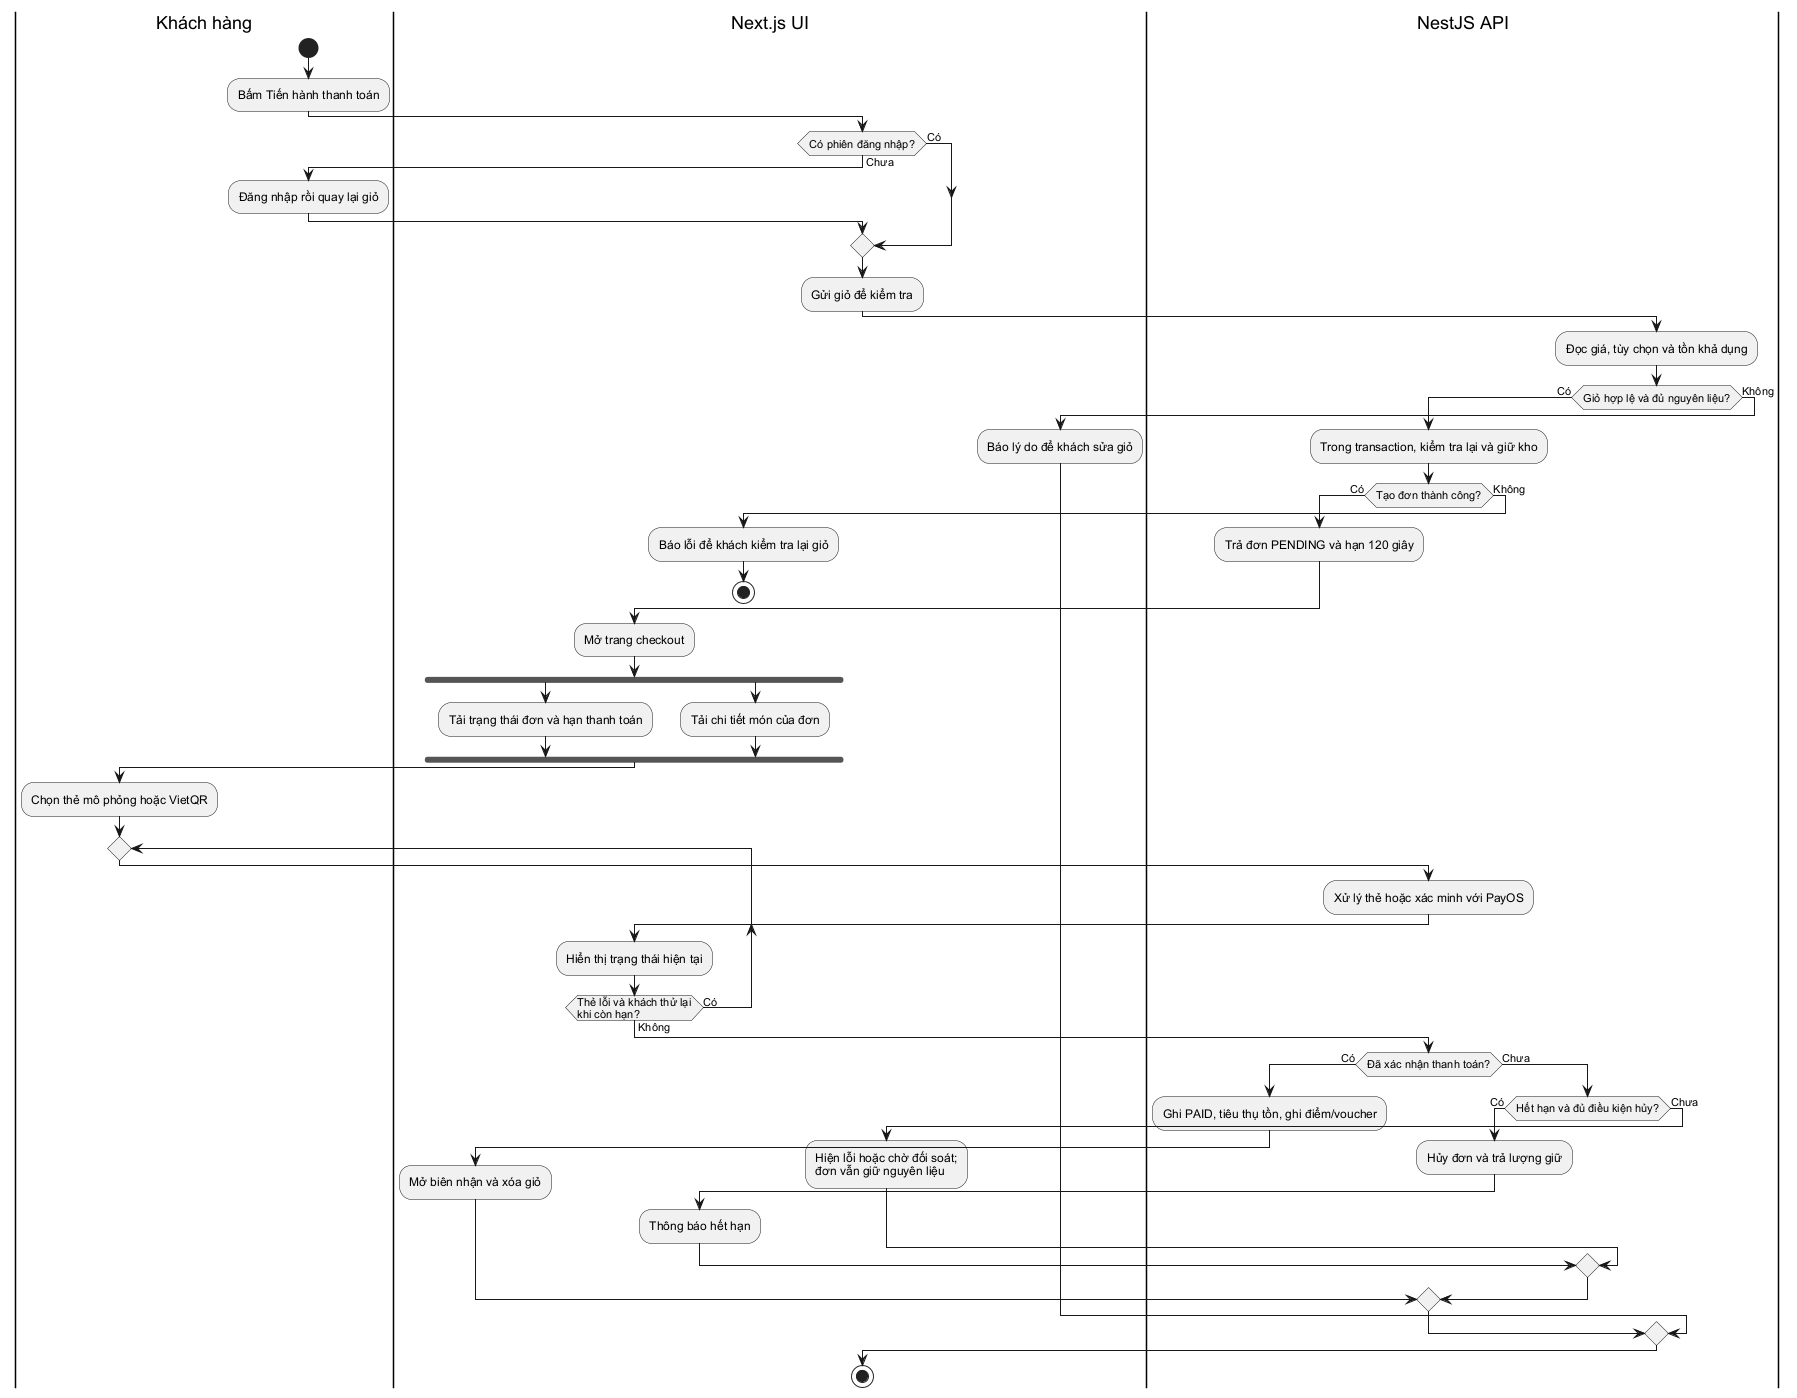
\includegraphics[width=\linewidth,height=0.70\textheight,keepaspectratio]{../../diagrams/activity-checkout-overview.png}\\[0.5em]
{\small\itshape Hình 2.1a. Hoạt động đặt và thanh toán đơn hàng}
\end{center}

\clearpage
\subsubsection{Kiểm tra giỏ và giữ nguyên liệu}
API kiểm tra giỏ ở chế độ chỉ đọc. Hai truy vấn món kèm giá và topping được khởi chạy cùng lúc. API chờ đủ hai kết quả trước khi đọc công thức. Khi tạo đơn, API tính giá và ưu đãi, sau đó kiểm tra lại giá và tăng lượng giữ bằng lệnh cập nhật có điều kiện đủ tồn trong transaction. Đơn, dòng món và lượng giữ được ghi cùng nhau. Khi thiếu nguyên liệu hoặc có lỗi ghi, transaction được hoàn tác.

\begin{center}
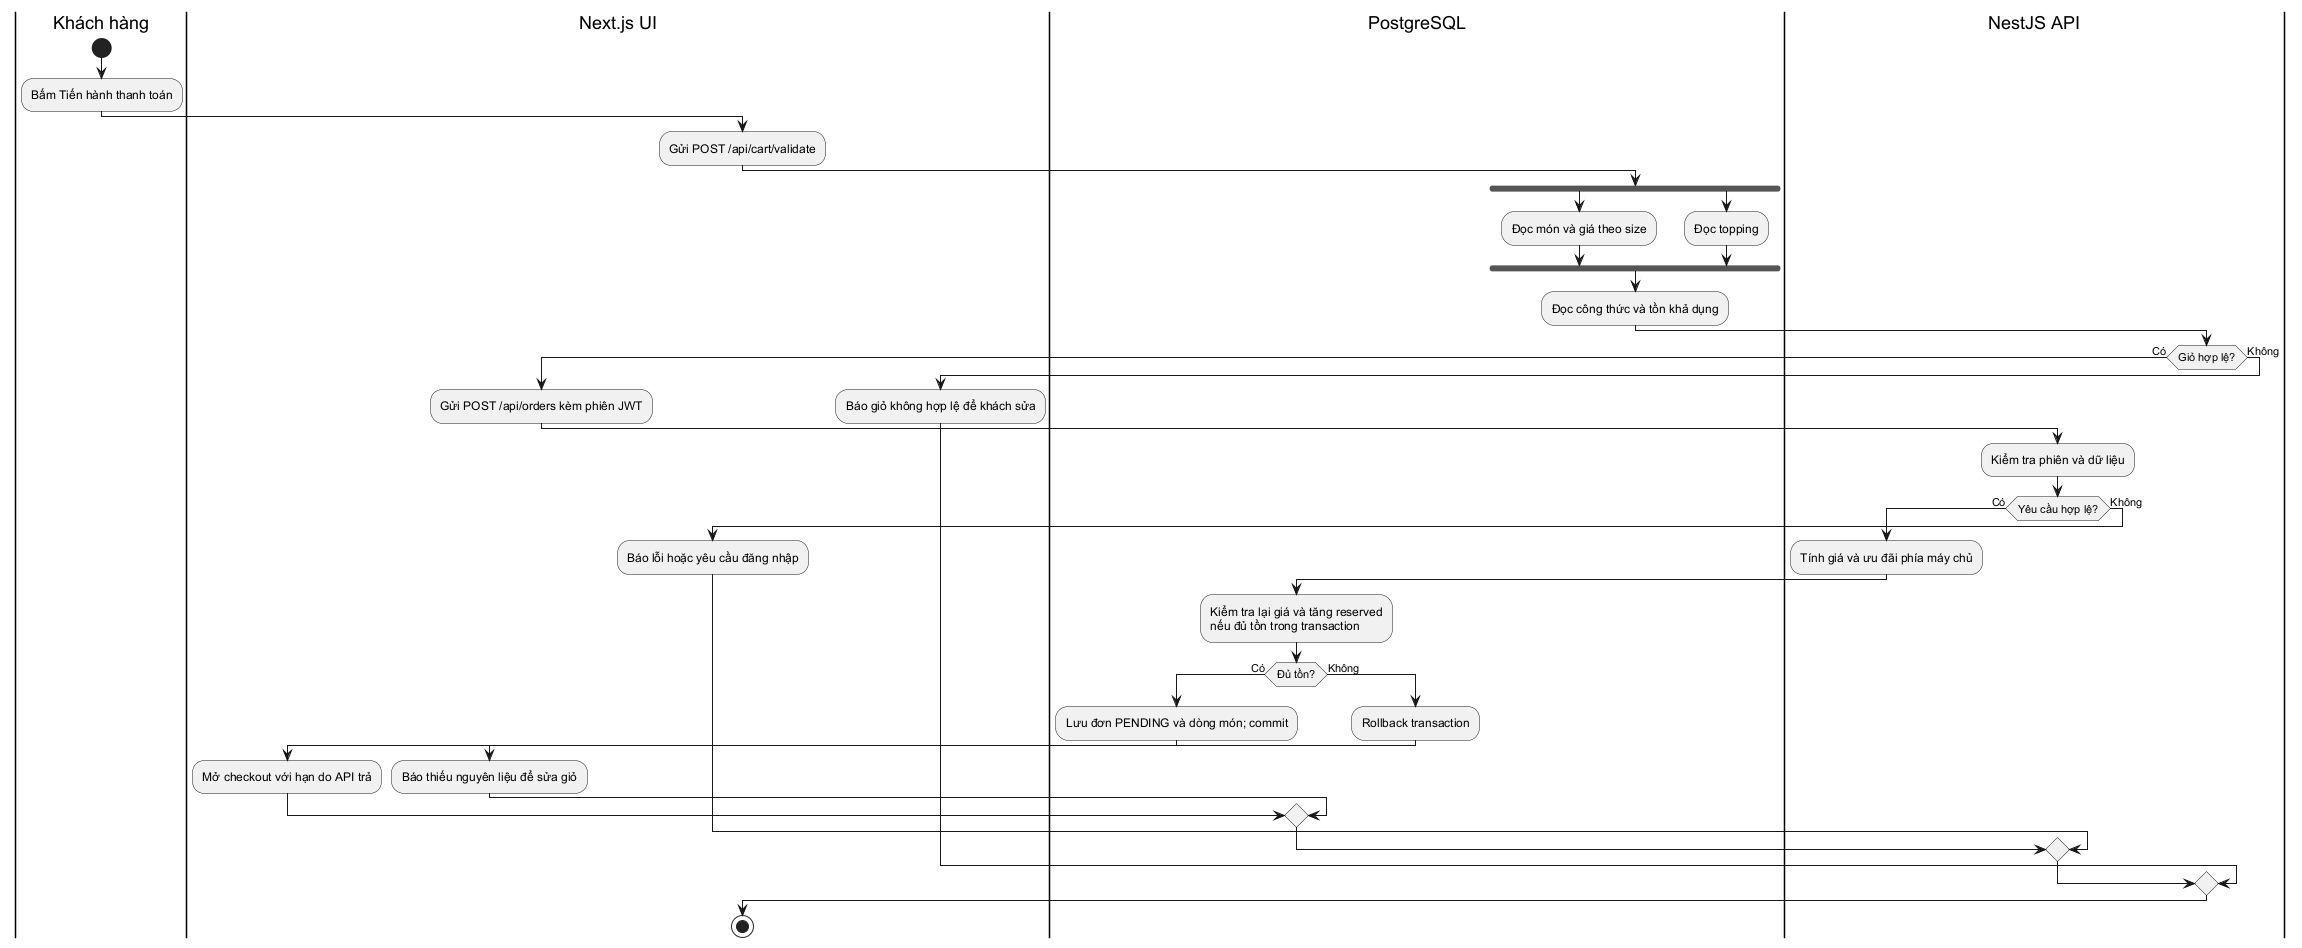
\includegraphics[width=\linewidth,height=0.70\textheight,keepaspectratio]{../../diagrams/activity-order-reservation.png}\\[0.5em]
{\small\itshape Hình 2.1b. Kiểm tra giỏ và giữ nguyên liệu}
\end{center}

\clearpage
\subsubsection{Thanh toán thẻ mô phỏng và chống xử lý lặp}
Khóa \texttt{Idempotency-Key} gắn với bản ghi \texttt{Payment}. Yêu cầu lặp trả kết quả đã ghi. Nếu thẻ thất bại, API ghi \texttt{FAILED}, đơn chuyển sang \texttt{PAYMENT\_FAILED} và giữ kho đến khi đơn được thanh toán hoặc đủ điều kiện hủy.

\begin{center}
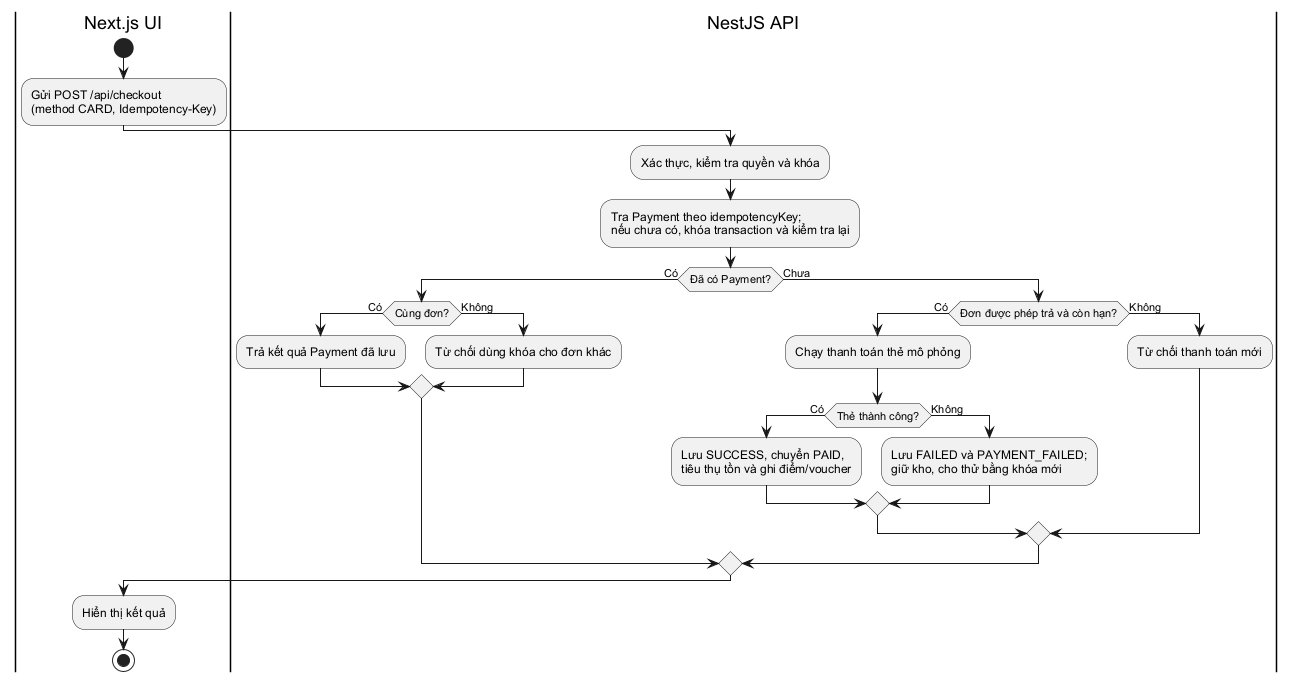
\includegraphics[width=\linewidth,height=0.70\textheight,keepaspectratio]{../../diagrams/activity-idempotency.png}\\[0.5em]
{\small\itshape Hình 2.1c. Xử lý thẻ mô phỏng}
\end{center}

\clearpage
\subsubsection{VietQR, webhook và đối soát}
Webhook có chữ ký hợp lệ hoặc kết quả đối soát trực tiếp có thể xác nhận đã nhận đủ tiền. Khi hết hạn, đơn có link PayOS chỉ được hủy và trả kho nếu link đã đóng và chưa nhận tiền. Nếu PayOS chưa xác nhận hoặc số tiền chưa khớp, API giữ nguyên đơn để đối soát.

\begin{center}
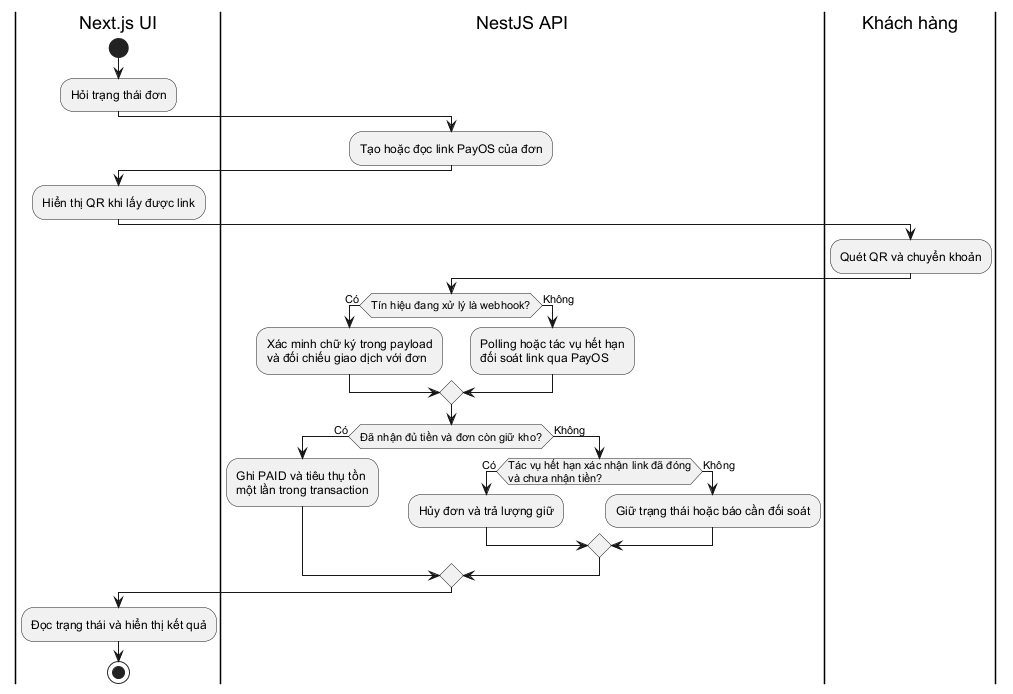
\includegraphics[width=\linewidth,height=0.70\textheight,keepaspectratio]{../../diagrams/activity-payos-webhook.png}\\[0.5em]
{\small\itshape Hình 2.1d. Xác minh giao dịch VietQR và xử lý hết hạn}
\end{center}

\clearpage
\subsection{Task 2.2 -- Sequence diagram}

\subsubsection{Luồng UC-01 từ giỏ đến biên nhận}
Năm lifeline gồm khách hàng, Next.js UI, NestJS API, PostgreSQL và PayOS. Sơ đồ thể hiện kiểm tra giỏ, tạo đơn với phiên JWT, transaction giữ nguyên liệu, hai nhánh thanh toán và kết quả hiển thị. Khi mở checkout, giao diện tải trạng thái và chi tiết đơn song song như trong Activity Diagram. Các khung tham chiếu dẫn đến sơ đồ chi tiết.

\begin{center}
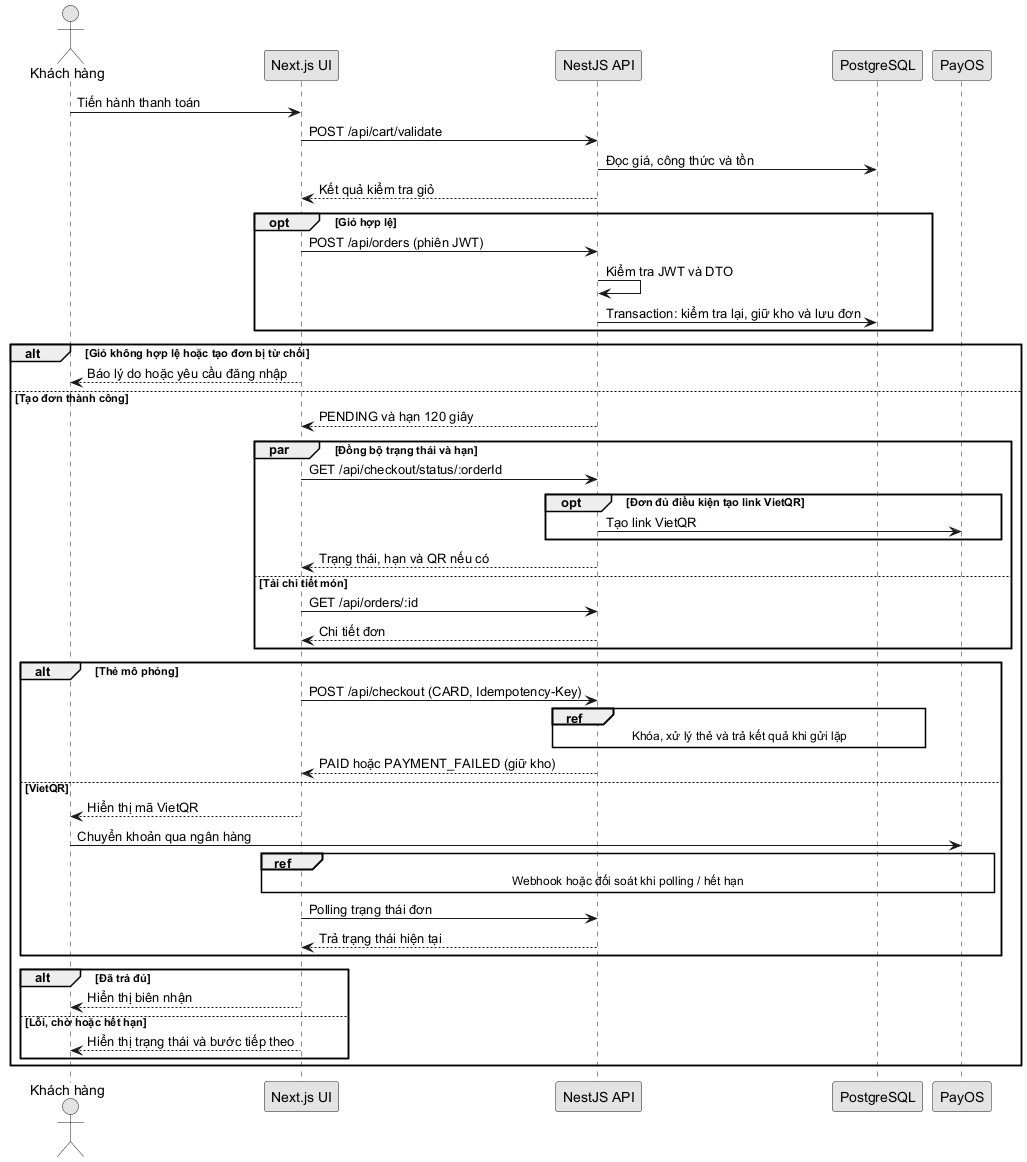
\includegraphics[width=\linewidth,height=0.70\textheight,keepaspectratio]{../../diagrams/sequence-checkout-overview.png}\\[0.5em]
{\small\itshape Hình 2.2a. Trình tự đặt và thanh toán đơn hàng}
\end{center}

\clearpage
\subsubsection{Tạo đơn và tạm giữ nguyên liệu}
Bước kiểm tra giỏ chỉ đọc dữ liệu. API tạo đơn yêu cầu JWT, kiểm tra DTO, tính giá và ưu đãi ở máy chủ, kiểm tra lại giá rồi giữ nguyên liệu bằng cập nhật có điều kiện trong transaction. API trả \texttt{id}, \texttt{total}, trạng thái \texttt{PENDING} và \texttt{reservationExpiresAt}.

\begin{center}
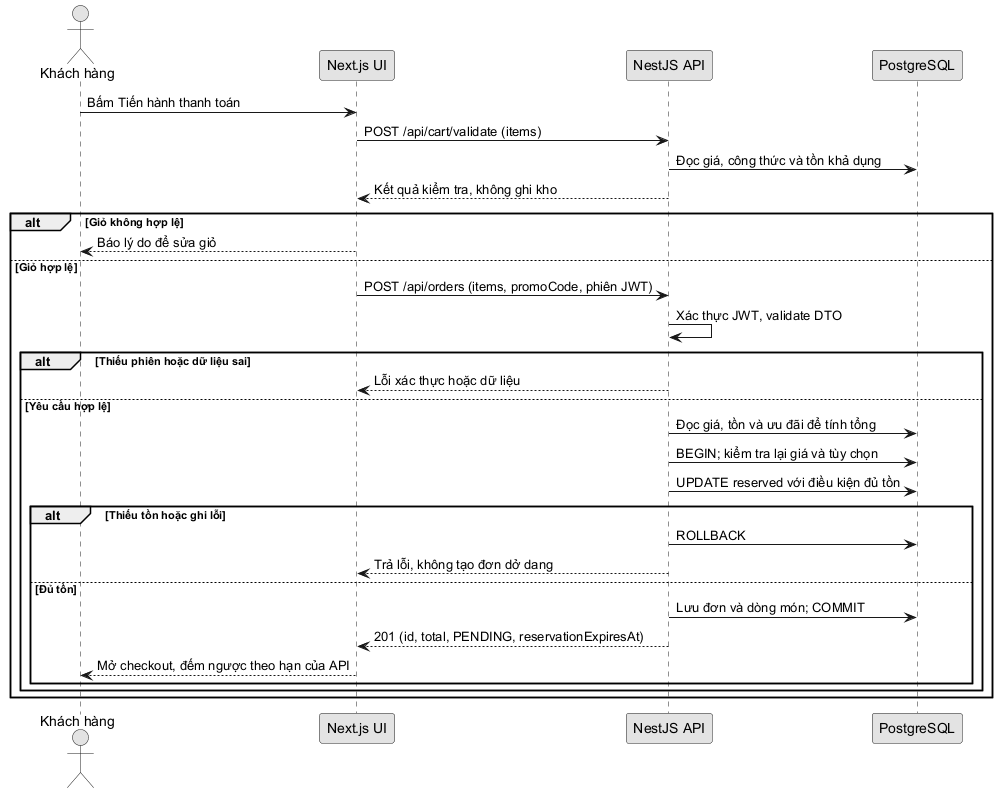
\includegraphics[width=\linewidth,height=0.70\textheight,keepaspectratio]{../../diagrams/sequence-order-reservation.png}\\[0.5em]
{\small\itshape Hình 2.2b. Kiểm tra dữ liệu, khóa nguyên liệu và tạo đơn}
\end{center}

\clearpage
\subsubsection{Chống xử lý lặp khi thanh toán thẻ}
API tra \texttt{Payment.idempotencyKey}. Nếu chưa có kết quả, transaction dùng khóa theo key và khóa dòng đơn, rồi kiểm tra lại để xử lý các yêu cầu đồng thời. Kết quả trả về dựa trên bản ghi \texttt{Payment}. Lượt thử sau thất bại dùng khóa mới nếu đơn còn hạn.

\begin{center}
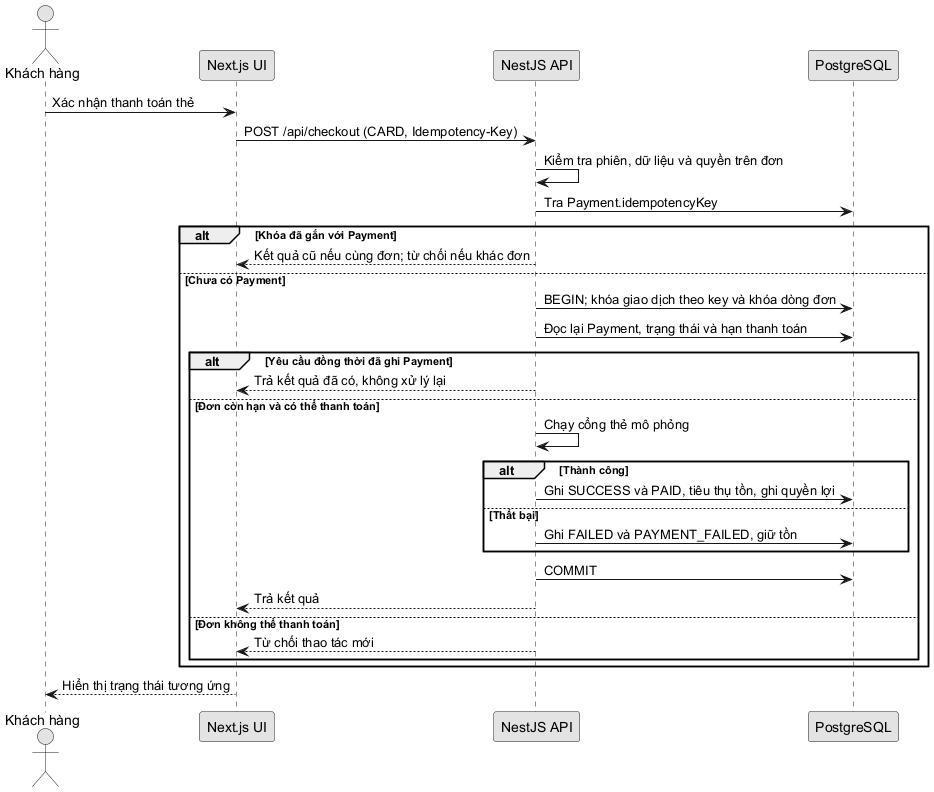
\includegraphics[width=\linewidth,height=0.70\textheight,keepaspectratio]{../../diagrams/sequence-idempotency.png}\\[0.5em]
{\small\itshape Hình 2.2c. Khóa transaction và trả lại kết quả đã ghi}
\end{center}

\clearpage
\subsubsection{Thanh toán VietQR và đối soát PayOS}
PayOS gửi webhook có \texttt{data} và \texttt{signature} trong body. API dùng SDK PayOS kiểm tra chữ ký và đối chiếu giao dịch với đơn. Polling hoặc tác vụ hết hạn cũng có thể đọc trực tiếp trạng thái link. Webhook hợp lệ và polling đồng thời chỉ hoàn tất đơn một lần.

\begin{center}
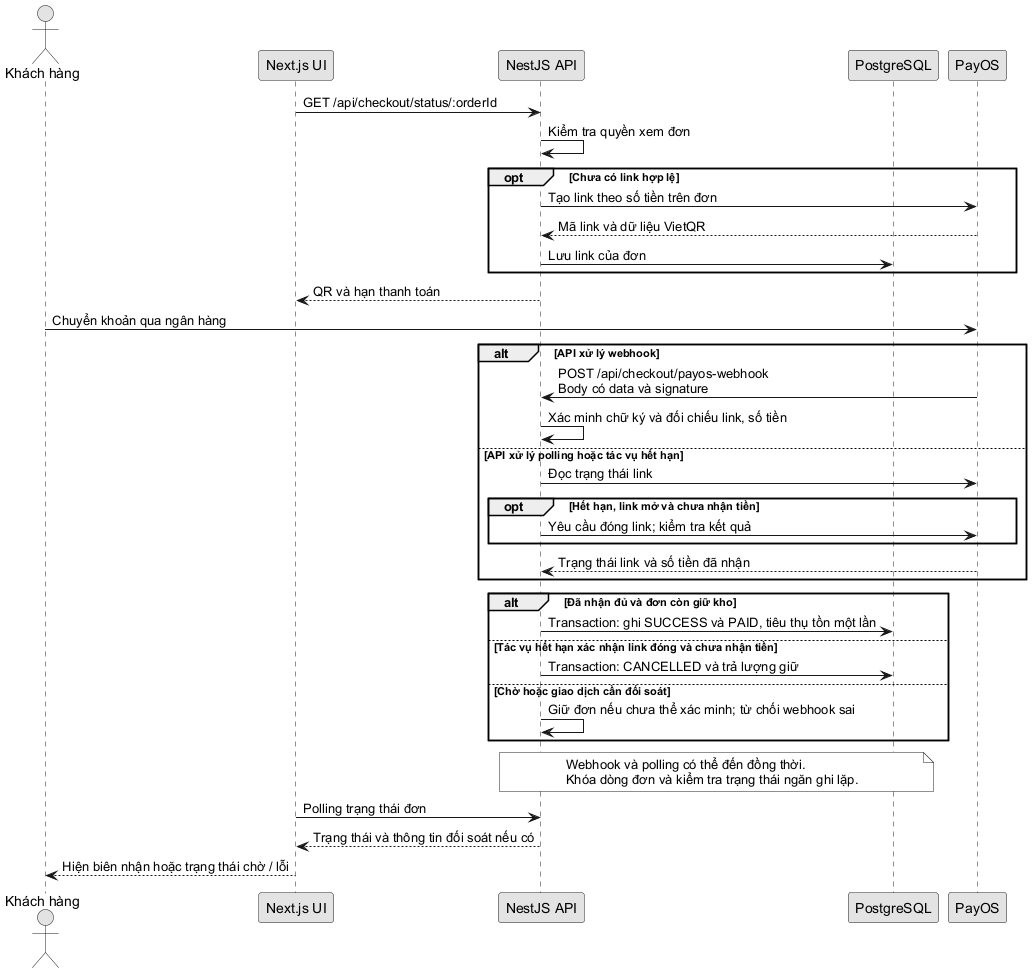
\includegraphics[width=\linewidth,height=0.70\textheight,keepaspectratio]{../../diagrams/sequence-payos-webhook.png}\\[0.5em]
{\small\itshape Hình 2.2d. Xác thực webhook, polling và đối soát khi hết hạn}
\end{center}

\subsection{Task 2.3 -- Class diagram}
\emph{Khung nội dung: nhóm sẽ bổ sung tạo phẩm và minh chứng của task này.}


% Task 3 -- Thiết kế kiến trúc
\section{Task 3 -- Thiết kế kiến trúc}
\subsection{Task 3.1 -- Phương pháp và quyết định kiến trúc}
\emph{Khung nội dung: nhóm sẽ bổ sung tạo phẩm và minh chứng của task này.}

\subsection{Task 3.2 -- Deployment diagram}
\emph{Khung nội dung: nhóm sẽ bổ sung tạo phẩm và minh chứng của task này.}


% Task 4 -- Triển khai Sprint 1
\section{Task 4 -- Triển khai Sprint 1}
\subsection{Task 4.1 -- Thiết lập repository}
\emph{Khung nội dung: nhóm sẽ bổ sung tạo phẩm và minh chứng của task này.}

\subsection{Task 4.2 -- Quản lý tài liệu}

Hồ sơ yêu cầu, mô hình hóa và kiến trúc được quản lý cùng mã nguồn trong
\nolinkurl{docs/}. Báo cáo LaTeX dùng \nolinkurl{docs/requirements/task1/main.tex}
để ghép các mục từ tệp con. Các tạo phẩm chi tiết được tổ chức như sau.

\begin{itemize}
  \item \textbf{Task 1} lưu bối cảnh và phạm vi, SRS và đặc tả use-case trong
        \nolinkurl{docs/requirements/}.
  \item \textbf{Task 2} lưu mã nguồn PlantUML và các bản xuất PNG/SVG của sơ đồ
        trong \nolinkurl{docs/diagrams/}. Báo cáo tham chiếu đến bản xuất tương ứng.
  \item \textbf{Task 3} lưu tài liệu kiến trúc và sáu ADR trong
        \nolinkurl{docs/architecture/}. \nolinkurl{docs/deployment.md}
        mô tả môi trường triển khai, migration và rollback.
\end{itemize}

Khi thay đổi yêu cầu, sơ đồ hoặc kiến trúc, pull request ghi lý do và cập nhật
các tạo phẩm bị ảnh hưởng. Với sơ đồ, cập nhật cả nguồn và ảnh kết xuất trong
cùng thay đổi. \nolinkurl{docs/traceability-matrix.md} liên kết mã yêu cầu với
use-case hoặc user story, thiết kế, API và ca kiểm thử.

\subsection{Task 4.3 -- MVP Sprint 1}
\emph{Khung nội dung: nhóm sẽ bổ sung tạo phẩm và minh chứng của task này.}

\subsection{Task 4.4 -- Continuous Integration}

Workflow \nolinkurl{.github/workflows/ci.yml} tự chạy khi mở hoặc cập nhật pull
request vào \texttt{main}. Hai job \texttt{Build \& Check Backend} và
\texttt{Build \& Check Frontend} dùng Node.js 22, cài phụ thuộc bằng
\texttt{npm ci}, rồi lần lượt chạy lint, unit test và build. Backend tạo
Prisma Client trước khi lint. Job \texttt{API integration and order E2E} dựng
PostgreSQL 16 tạm, áp migration và chạy test tích hợp cùng E2E qua API.

\paragraph{Minh chứng trên PR thanh toán}
\begin{itemize}
  \item \href{https://github.com/PhucTruong11/brewlite-assignment2/pull/1}{PR \#1}
        tích hợp nhánh \texttt{payments} vào \texttt{main}.
  \item \href{https://github.com/PhucTruong11/brewlite-assignment2/actions/runs/42744381085}{CI lượt \#6}
        phát hiện lỗi ở bước \texttt{npm ci} của hai job dùng API, tại commit
        \texttt{7438dd1}.
  \item \href{https://github.com/PhucTruong11/brewlite-assignment2/actions/runs/42769688179}{CI lượt \#7}
        đạt cả ba job sau khi cập nhật \nolinkurl{apps/api/package-lock.json}
        ở commit \texttt{f5dcc2d}.
\end{itemize}

GitHub hiện báo \texttt{main} chưa được bảo vệ. Để đáp ứng tiêu chí chặn merge
khi CI thất bại, cần bật branch protection hoặc ruleset trên \texttt{main} và
đặt cả ba job trên làm required checks. Quality gate của workflow phát hành
đã chặn bước triển khai nếu CI thất bại.


% Task 5 -- Triển khai Sprint 2, CI/CD và bàn giao
\section{Task 5 -- Triển khai Sprint 2 và bàn giao}
\subsection{Task 5.1 -- Hoàn thiện MVP}
\emph{Khung nội dung: nhóm sẽ bổ sung tạo phẩm và minh chứng của task này.}

\subsection{Task 5.2 -- Tích hợp và kiểm thử}
\emph{Khung nội dung: nhóm sẽ bổ sung tạo phẩm và minh chứng của task này.}

\subsection{Task 5.3 -- Continuous Delivery/Deployment}

Workflow \nolinkurl{.github/workflows/cd.yml} tự chạy khi có push vào
\texttt{main}, bao gồm commit sau khi merge PR. Workflow cũng hỗ trợ tag
\nolinkurl{v*} và chạy thủ công. Các bước phát hành chạy theo thứ tự sau.

\begin{enumerate}[leftmargin=*]
  \item \textbf{Quality gate.} Gọi lại CI trên cùng commit để chạy lint,
        unit test, build, kiểm thử tích hợp và E2E. Chỉ chuyển sang đóng gói
        khi toàn bộ job kiểm tra đạt.
  \item \textbf{Đóng gói.} Build hai Docker image web và API, gắn tag bằng
        commit SHA và đẩy lên GitHub Container Registry.
  \item \textbf{Kiểm tra đích và migration.} Dùng secrets từ GitHub
        Environment \texttt{production}. Kiểm tra đích Render/Vercel và xác
        nhận baseline migration cùng bản sao lưu. Sau đó chạy
        \texttt{prisma migrate deploy} trên Supabase.
  \item \textbf{Deploy và smoke test.} Render triển khai API từ SHA phát hành.
        Vercel CLI triển khai web từ cùng checkout. Workflow kiểm tra
        \nolinkurl{/api/health}, \nolinkurl{/api/products}, trang web HTTPS và
        health endpoint qua proxy web. Image GHCR lưu bản đóng gói theo SHA
        để truy vết.
\end{enumerate}

Nếu rollout lỗi sau khi đã cập nhật một ứng dụng, workflow thử khôi phục bản
Vercel trước đó hoặc commit Render trước đó, tùy bước đã thành công. Rollback
schema và dữ liệu PostgreSQL được xử lý riêng theo
\nolinkurl{docs/deployment.md}.
\href{https://github.com/PhucTruong11/brewlite-assignment2/actions/runs/43011669621}{Lượt phát hành của commit \texttt{55e5bbe}}
ghi nhận CI, publish image, migration, deploy và smoke test đều đạt.

\subsection{Task 5.4 -- Triển khai và bàn giao}

\begin{itemize}
  \item \textbf{Mã nguồn trên GitHub}
        \url{https://github.com/PhucTruong11/brewlite-assignment2}.
  \item \textbf{Web production}
        \url{https://brewlite-frontend.vercel.app/}.
  \item \textbf{API production}
        \url{https://brewlite-api-omni.onrender.com/api}.
  \item \textbf{Health check trực tiếp}
        \url{https://brewlite-api-omni.onrender.com/api/health}.
  \item \textbf{Health check qua web}
        \url{https://brewlite-frontend.vercel.app/api/health}.
\end{itemize}

Kiểm tra ngày 13/11/2026 ghi nhận HTTP 200 ở trang web, API health, API
danh sách món và health check qua proxy web.

Web Next.js chạy trên Vercel và gọi API NestJS trên Render qua proxy cùng
origin. Render kết nối PostgreSQL Supabase qua TLS bằng thông tin xác thực.
Trình duyệt truy cập dữ liệu qua API. Cấu hình production và bí mật nằm trong
các môi trường của Render, Vercel và GitHub Actions. Repository cung cấp tệp
mẫu để chỉ ra tên biến cần cấu hình. Log CD dùng để đối chiếu kết quả migration,
deploy và smoke test.

\paragraph{Hướng dẫn tái tạo và demo}
Người nghiệm thu có thể clone repository, dùng \nolinkurl{README.md} để xem
lệnh test và build, dùng \nolinkurl{docker/README.md} để khởi động web, API và
PostgreSQL local, và dùng \nolinkurl{docs/deployment.md} để xem quy trình
release và rollback. Kịch bản demo đi từ menu đến chọn size/topping, kiểm
tra giỏ, đăng nhập, tạo đơn, thanh toán CARD mô phỏng, mở biên nhận và kiểm
tra lịch sử đơn. Có thể trình bày thêm luồng VietQR khi kênh PayOS đã cấu hình.

\paragraph{Minh chứng bàn giao}
Phiên bản production đối chiếu được theo commit \texttt{55e5bbe} và
\href{https://github.com/PhucTruong11/brewlite-assignment2/actions/runs/43011669621}{log phát hành}.
Tag phiên bản và release notes chưa thấy trên GitHub. Link video hoặc biên
bản demo trực tiếp, Sprint Review và Sprint Retrospective cần đính kèm khi
nộp nếu nhóm đã có các tài liệu này. Cấu hình giới hạn mạng của Supabase
cần được xác nhận từ dashboard dự án.

\end{document}
